\documentclass[11pt]{article}
\usepackage{tutorial-students}
\usepackage{tikz}
\usepackage{tkz-graph}

\newcommand{\fillinMCmath}[1]{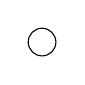
\begin{tikzpicture}\draw circle [radius=0.5em];\end{tikzpicture}\ #1}
\newcommand{\fillinMCmathsoln}[1]{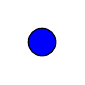
\begin{tikzpicture}\draw[black, fill=blue] circle [radius=0.5em];\end{tikzpicture}\ #1}

\author{}
\date{}
\begin{document}

\title{CPSC 320 2021W1: Assignment 2}

\maketitle
\vspace{-0.5in}

This assignment is due on \textbf{Monday, Oct 4 at 10pm Vancouver time} on Gradescope. Assignments submitted within 24 hours after the deadline will be accepted, but a penalty of 15\% will be applied. Please follow the guidelines provided in Assignment 1.

All the submission and formatting rules for Assignment~1 apply to
this assignment as well.  For drawings of graphs, however, we will permit
pictures of hand-drawn graphs included in your PDF submission, as we did
with pseudocode on the last assignment, as long as they are clear and
easy-to-mark.

%------------------------------------------------------------------------------------
\section{List of names of group members (as listed on Canvas)}

Provide the list here. This is worth 1 mark. Include student numbers
as a secondary failsafe if you wish.

\begin{soln}
Mathew Balsdon 21041694 \\
Michael Woolsey 87234621
\end{soln}

\section{Statement on collaboration and use of resources}
To develop good practices in doing homeworks,
citing resources and acknowledging input from others, please complete the following.
This question is worth 2 marks.

\begin{enumerate}
\item All group members have read and followed the guidelines for groupwork
on assignments given on the website (see \url{https://www.students.cs.ubc.ca/~cs-320/2021S2/coursework.html}, under Assignments).
\fillinMCmathsoln{Yes} \hspace{.5in} \fillinMCmath{No}

\item We used the following resources (list books, online sources, etc. that you consulted):

\begin{soln}
CPSC 320 Piazza \\
https://en.wikipedia.org/wiki/Directed\_acyclic\_graph \\
https://en.wikipedia.org/wiki/Bipartite\_graph \\
Jon Kleinberg, Éva Tardos - Algorithm Design-Pearson (2006)
\end{soln}
\item One or more of us consulted with course staff during office hours.

\fillinMCmath{Yes} \hspace{.5in} \fillinMCmathsoln{No}

\item One or more of us collaborated with other CPSC 320 students; none of us took
      written notes during our consultations and we took at least a half-hour break afterwards.

\fillinMCmath{Yes} \hspace{.5in} \fillinMCmathsoln{No}

      If yes, please list their name(s) here:


\item One or more of us collaborated with or consulted others outside of CPSC 320; none of us took written notes during our consultations and we took at least a half-hour break afterwards.

\fillinMCmath{Yes} \hspace{.5in} \fillinMCmathsoln{No}

      If yes, please list their name(s) here:

\end{enumerate}
\newpage

\section{Puzzling Over Graphs}

When first learning graph theory, it's most intuitive to start with small
examples that are easy to draw and see.  However, in real applications,
the graphs are generally too large to visualize, and often correspond
to abstract concepts or logical relations.  This question aims to help
you practice that transition.

\begin{enumerate}
\item (1 mark)
We'll start with creating a graph for the classic Wolf-Goat-Cabbage puzzle.
See the Wikipedia page (or other online resources) at
\url{https://en.wikipedia.org/wiki/Wolf,_goat_and_cabbage_problem} if
you are unfamiliar with this puzzle.  Imagine a graph where the
vertices represent possible states of the puzzle, e.g., you start in
a vertex that represents the person, wolf, goat, and cabbage all on the
left side of the river, and you are trying to reach the vertex that
represents the person, wolf, goat, and cabbage all on the right side of
the river.  We've drawn all 16 possible vertices below, using notation
like ``PWC-G'' to indicate that the person (P), wolf (W), and cabbage (C)
are on the left bank of the river, but the goat (G) is on the right bank.
\begin{center}
\footnotesize % Makes text smaller, so figure will be smaller
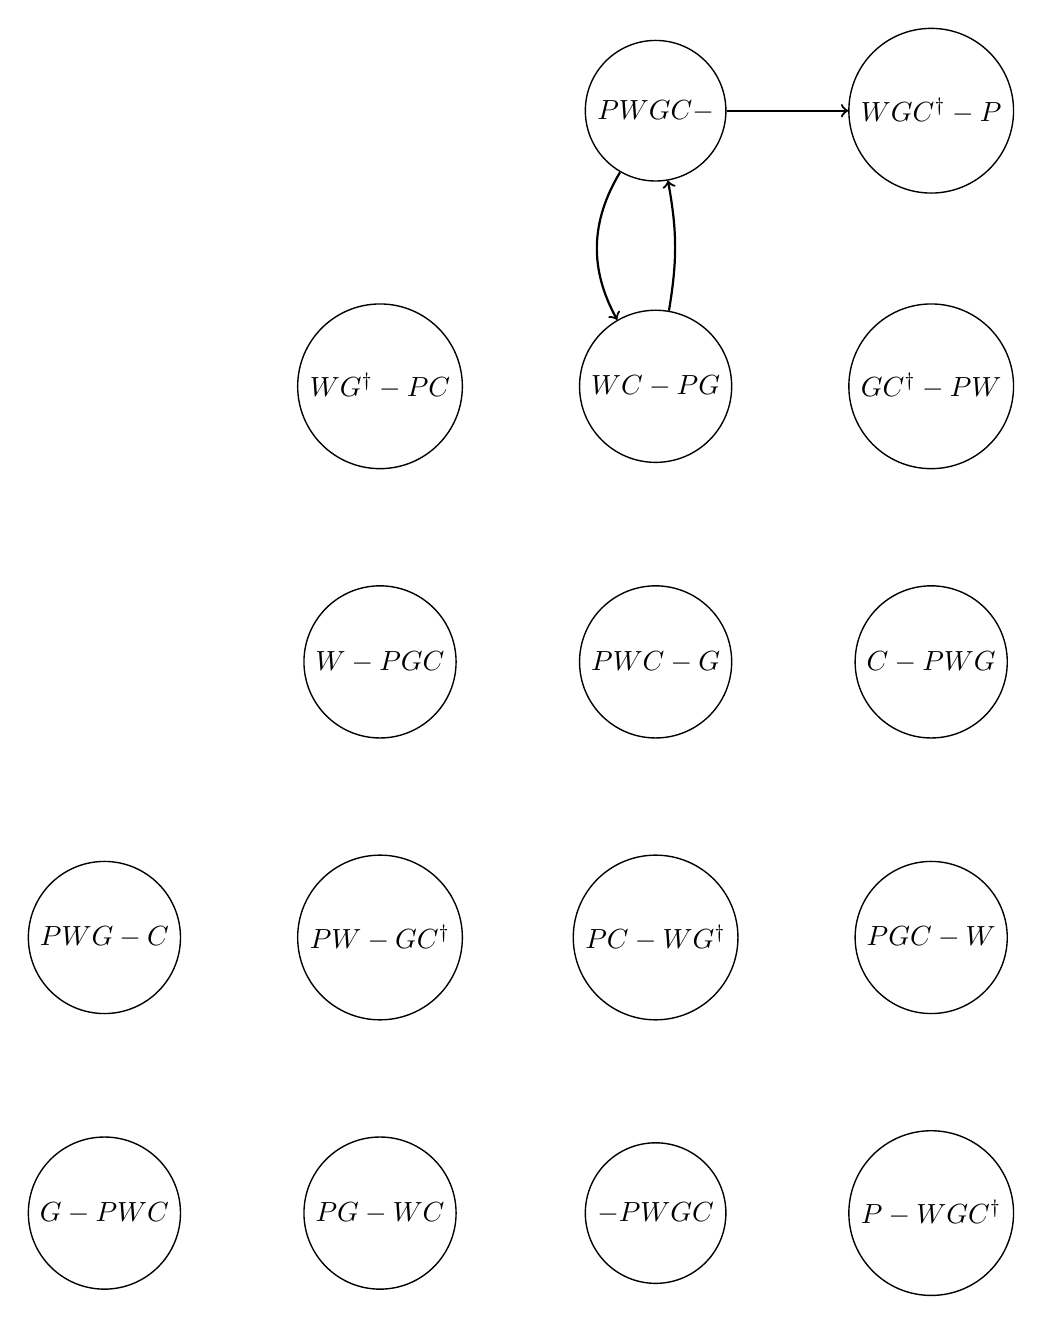
\begin{tikzpicture}[scale=1]
\GraphInit[vstyle=Normal]
%\SetUpEdge[lw = 1.5pt]
\SetGraphUnit{3.5}
% First row of vertices
\Vertex[L=$PWGC-$]{PWGC-}
\EA[L=$WGC^\dagger-P$](PWGC-){WGC-P}
% Second row
\SOWE[L=$WG^\dagger-PC$](PWGC-){WG-PC}
\SO[L=$WC-PG$](PWGC-){WC-PG}
\SOEA[L=$GC^\dagger-PW$](PWGC-){GC-PW}
% Third row
\SOWE[L=$W-PGC$](WC-PG){W-PGC}
\SO[L=$PWC-G$](WC-PG){PWC-G}
\SOEA[L=$C-PWG$](WC-PG){C-PWG}
% Fourth row
\SOWE[L=$PWG-C$](W-PGC){PWG-C}
\SO[L=$PW-GC^\dagger$](W-PGC){PW-GC}
\SO[L=$PC-WG^\dagger$](PWC-G){PC-WG}
\SOEA[L=$PGC-W$](PWC-G){PGC-W}
% Last row
\SO[L=$G-PWC$](PWG-C){G-PWC}
\EA[L=$PG-WC$](G-PWC){PG-WC}
\EA[L=$-PWGC$](PG-WC){-PWGC}
\EA[L=$P-WGC^\dagger$](-PWGC){P-WGC}

%%% Add your edges below
\Edges[style={->}](PWGC-,WGC-P)			% default straight arrow
\Edges[style={->,bend right}](PWGC-,WC-PG)	% default bent arrow
\Edges[style={->,bend right=10}](WC-PG,PWGC-)	% You can adjust amount of bend
\end{tikzpicture}
\end{center}
Your job is to draw in all the missing directed edges in this graph, where an
edge should go from state $x$ to state $y$ if it's possible to
transition from $x$ to $y$ via one legal river crossing.  We've
drawn the first few edges to get you started.  Note that we have marked
illegal states (ones where something is going to get eaten!) with
the symbol $\dagger$, and those states should have no outgoing edges.

\begin{soln}
Here is our solution:\\
\includegraphics[width=365px]{unknown.png}
\end{soln}

\item (1 mark)
If you considered all the edges to be undirected, would the graph for
Wolf-Goat-Cabbage be a tree?  Briefly justify your answer.

\begin{soln}
No, as in this case, the graph would have cycles, which breaks the definition of a tree, so it cannot be a tree
\end{soln}

\item (1 mark)
Is the graph for Wolf-Goat-Cabbage a DAG (directed acyclic graph)?
Briefly justify your answer.

\begin{soln}
No, as there are cycles! For example, we can go between any two 'non-terminating' nodes as much as we want.
\end{soln}

\item (1 mark)
Explain why the graph for Wolf-Goat-Cabbage is bipartite (even if
it doesn't look like it).

\begin{soln}
Let the set $U$ consist of nodes $\{(PWGC-), (PWC-G), (PWG-C), (PW-GC\dagger), (PC-WG\dagger), (PGC-W), (PG-WC), (P-WGC\dagger)\}$, and let the set $V$ contain all other nodes. Then, there is an edge connecting any node in one set to a node in the other, and there are no edges between nodes in a set, as per the definition of a bipartite graph.
\end{soln}

\item (1 mark)
Assume you are using depth-first search (DFS),
starting from vertex $PWGC-$,
and trying to reach the goal vertex $-PWGC$ (stopping when the node is found).
In the \textbf{best case},
how many edges does the algorithm explore?
(The algorithm ``explores'' an edge when it follows an edge from
one vertex to another, even if the edge leads to a vertex that
was visited already or is illegal.
Using the pseudocode of the textbook, we count an edge when it
is in the loop ``\texttt{For each edge $(u,v)$ incident to $u$}'')
(Do not worry too much if you miscount by a few edges.)

\begin{soln}
There are 8 nodes (in this order):\\ $(PWGC-),(WC-PG),(PWC-G),(W-PGC),(PWG-C),(G-PWC),(PG-WC),(-PWGC)$\\
This means we explore 7 edges.
\end{soln}

\item (1 mark)
Assume you are using depth-first search (DFS),
starting from vertex $PWGC-$,
and trying to reach the goal vertex $-PWGC$.
In the \textbf{worst case},
how many edges does the algorithm explore?
(Do not worry too much if you miscount by a few edges.) 

\begin{soln}
There will be 25 different edges!
\end{soln}

\item (1 mark)
Assume you are using breadth-first search (BFS),
starting from vertex $PWGC-$,
and trying to reach the goal vertex $-PWGC$.
In the \textbf{best case},
how many edges does the algorithm explore?
(Do not worry too much if you miscount by a few edges.)

\begin{soln}
There will be 20 different edges!
\end{soln}

\item (1 mark)
Assume you are using breadth-first search (BFS),
starting from vertex $PWGC-$,
and trying to reach the goal vertex $-PWGC$.
In the \textbf{worst case},
how many edges does the algorithm explore?
(Do not worry too much if you miscount by a few edges.)

\begin{soln}
There will be 26 different edges!
\end{soln}

\item (4 marks)
Redo the preceding 4 parts (DFS best case, DFS worst case, BFS best case,
BFS worst case), assuming that you start from the vertex
$PG-WC$ instead (but with the same goal vertex of $-PWGC$).

\begin{soln}
DFS best case: 1
DFS worst case: 26
BFS best case: 2
BFS worst case: 5
\end{soln}

\item (1 mark)
Now, let's consider a different puzzle:  Sudoku.
See the Wikipedia page (or other online resources) at
\url{https://en.wikipedia.org/wiki/Sudoku} if
you are unfamiliar with this puzzle.
Let there be a vertex for every possible Sudoku board (including illegal ones),
i.e., for
every possible way of filling in a $9\times 9$ board with the numbers
from $1,\ldots, 9$ or leaving the square blank.
An edge will go from a vertex $x$ to a vertex $y$ if it's possible to
fill in \textbf{one digit} on $x$ to become $y$.
Draw the graph for Sudoku... haha, just kidding!  How many vertices are
in this graph?  The current estimate for the total number of photons
ever to exist in the universe is $4\times 10^{84}$.  How does that compare
to the size of this graph?

\begin{soln}
Each of the 81 boxes have 10 different states (either being empty or filled with 1-9's), so this is a normal combination problem. Meaning that the board has $10^{81}$ different possible states. There are about as many groups of 1000 photons in the entire universe there is 1 possible state for a sudoku board.
\end{soln}
\newpage
\item (1 mark)
If you considered all the edges to be undirected, would the graph for
Sudoku be a tree?  Briefly justify your answer.

\begin{soln}
No. If we were to write out every possible move, several nodes can point to the same board.
Assume this is the top left corner of the board:
\begin{center}
\begin{tabular}{|l|l|}
\hline
\hspace{1mm} & \hspace{1mm} \\ \hline
\hspace{1mm} & \hspace{1mm} \\ \hline
\end{tabular}
\end{center}
If we wanted to get to the following board:
\begin{center}
\begin{tabular}{|l|l|}
\hline
1 & \hspace{1mm} \\ \hline
\hspace{1mm} & 2 \\ \hline
\end{tabular}
\end{center}
We could either start out with a move like
\begin{center}
\begin{tabular}{|l|l|}
\hline
1 & \hspace{1mm} \\ \hline
\hspace{1mm} & \hspace{1mm} \\ \hline
\end{tabular}
\end{center}
Or the move
\begin{center}
\begin{tabular}{|l|l|}
\hline
\hspace{1mm} & \hspace{1mm} \\ \hline
\hspace{1mm} & 2 \\ \hline
\end{tabular}
\end{center}

This means our graph would start out from the same blank board, and have two different branches that ended up at the same exact board position (and each unique board position is its own unique vertex), meaning this would not have a tree shape

\end{soln}

\item (1 mark)
Is the graph for Sudoku a DAG (directed acyclic graph)?
Briefly justify your answer.

\begin{soln}
Assuming we cannot change or erase a number once it has been placed, the graph $is$ a DAG. Since we can't change a number or erase, the only thing we can do is add numbers, we cannot "go back" once we have placed a number. The only way we could get a cycle is if we were able to change back to a previous state, which is impossible. So our graph is a DAG. 
\end{soln}

\item (1 mark)
Is the graph for Sudoku bipartite?
Briefly justify your answer.

\begin{soln}
Yes, as we could have all states with an even number of boxes filled in one set, and all states with an odd number of boxes filled in another set. Since we can only add one number at a time, we will always hop between these two sets, meaning this graph is bipartite.
\end{soln}

\item (1 mark)
Which would work better, BFS or DFS, to solve Sudoku?
You should assume that partially-filled illegal boards (i.e., boards
that aren't completely filled, but already
have the same digit appearing more than once in a row, column,
or zone) have zero outdegree.

\begin{soln}
DFS will be superior to BFS for this case, as BFS will constantly be checking obviously incorrect solutions (such as filling every row that already has a 1 in it with 1's), whereas DFS will be able to tunnel down very fast, meaning that it should be able to spend less time checking obviously incorrect solutions.
\end{soln}

\end{enumerate}

\newpage
\section{Lexicographically ordered permutations: Runtime analysis part 1}

 The following definitions are exactly as in the first tutorial.
  Let $\pi[1..n]$ and $\pi'[1..n]$ be two permutations over a set of
$n$ integers. We say that $\pi < \pi'$ if and only if
for some $i$, $1\le i < n$,
\begin{equation}
\label{lessthan}
\pi[1..i-1] = \pi'[1..i-1] \mbox{ and } \pi[i] < \pi'[i].
\end{equation}
For example, if the set of integers is $\{1,5,6,8\}$, then
$5168 < 5618$ (the conditions hold with $i=2$), and also
$5168 < 5186$  (the conditions hold with $i=3$).

Let $\pi_1, \ldots, \pi_{n!}$ be an ordering of all $n!$ permutations
of a set of $n$ integers. This is a \emph{lexicographic ordering} if
$\pi_k < \pi_{k+1}$ for all $k, 1 \le k < n!$.

The tutorial solution describes criteria for
determining if one permutation $\pi'[1..n]$ of a set of $n$ integers
directly follows permutation
$\pi[1..n]$ in lexicographic order:
Find the smallest value, say $i$, in the range
$[0..n-1]$ such that $\pi[i+1..n]$ is sorted in descending order.
If $i=0$, $\pi$ must be the last permutation in lexicographic order,
so $\pi'$ cannot follow $\pi$.

Otherwise, if $i \ge 1$, 
find $j$, where $\pi[j]$ is the smallest value in $\pi[i+1..n]$ that
is larger than $\pi[i]$.
Then $\pi'$ follows $\pi$ in lexicographic order if and only if
\begin{enumerate}
\item
  $\pi'[1..i-1]$ = $\pi[1..i-1]$,
\item
  $\pi'[i] = \pi[j]$, and
\item  
  $\pi'[i+1..n]$ is sorted in ascending order.
\end{enumerate}

Using these criteria, the algorithm below takes
as input a permutation $p[1..n]$ of a set of
$n$ integers, and updates $p[1..n]$ to be the next permutation in lexicographic order. For example, if $p[1..4]$ is initially $7325$, then when
the algorithm completes, $p[1..4]$ should be $7352$.  If
there is no lexicographically next permutation, then $p$
remains unchanged.

\vspace{.2in}

\begin{algorithmic}[1]
\Procedure{Generate-Lexicographically-Next-Permutation}{$p[1..n]$}
\State $\triangleright$ $p[1..n]$ is a permutation of $n$ distinct integers
\State $\triangleright$ update $p[1..n]$ to be the lexicographically next permutation
\State $\triangleright$ leave $p[1..n]$ unchanged if there is no lexicographically next permutation
\State
\State $\triangleright$ find $i \in [0..n- 1]$ such that $p[i + 1..n]$ is sorted in descending order,
\State $\triangleright$ and either $i=0$ or $p[i] < p[i+1]$
\State $i = n-1$
\While{($i \ge 1$) AND ($p[i] > p[i+1]$)}
   \State $i \leftarrow i-1$
   \EndWhile
\State   
\State $\triangleright$ if $i=0$, there is no lexicographically next permutation; do nothing.
\If{$i>0$}
\State $\triangleright$ find $j$, where $p[j]$ is the smallest value in $p[i + 1..n]$ that is larger than $p[i]$
   \State $j \leftarrow i+1$
   \While{($j<n$) AND ($p[j+1] > p[i]$)}
      \State $j \leftarrow j+1$
   \EndWhile
\State
   \State swap the entries $p[i]$ and $p[j]$
   \State reverse the entries in $p[i+1..n]$ \hspace{.3in} $\triangleright$ so that they are in ascending order
\EndIf
\EndProcedure
\end{algorithmic}

\newpage
\begin{enumerate}
\item (1 mark)
If the input to the algorithm is 
$p[1..7] = 4567321$, 
what is the value of the array $p[1..7]$ when the algorithm completes?
No justification needed.\\
\begin{soln}
4571236
\end{soln}


\item
(2 marks)
Explain why the algorithm takes $\Theta(n)$ time in the worst case.

\begin{soln}
The first while loop (lines 9-10) is $\Theta(n)$, since we will start searching at the right of $p[1..n]$, and in the worst case i could be 1, so we would have to check every position of p until we get to one, which is n iterations. Once we are here, it is possible that our value of j could be $j=n$ (a situation where i=1 and j=n is a number like 1432, where the smallest number in p is on the left, then the rest of the numbers are in descending number), which means we will have it iterate the while loop at lines 16-17 about $n$ times. The swap (line 19) will be constant time, and here the reversing at line 20 will be $\Theta(n)$. This means we have around $\Theta(3n)$ operations, which is in $\Theta(n)$.
\end{soln}

\item (1 mark)
Describe an input on which the algorithm runs in $O(1)$ time.

\begin{soln}
An input where the algorithm runs in $O(1)$ time is when the last number $p[n]$ is larger than the second last number $p[n-1]$, i.e. $p[n] > p[n-1]$. An example is 3214. In a situation like this, we will set $i=3$ at line 8, then immediately breaking out of the while loop, then at line 15, we set $j=4$ and it will not even iterate the loop once, since $j=n$. The swap will be in constant time, and the reversal of the entries will not even occur since we just need to reverse $p[n..n]$.
\end{soln}

\end{enumerate}

\newpage

\section{Lexicographically ordered permutations: Runtime analysis part 2}

We can generate all permutations by calling
algorithm \textsc{Generate-Lexicographically-Next-Permutation}
$n!$ times: On the first call, the input is $p[1..n] = 12..n$, and on subsequent calls, the input is the value of $p[1..n]$ at the end of the previous call. Since the algorithm takes $\Theta(n)$ time in the worst case, and it is called $n!$ times, we know that the overall runtime is $O(n! \times n)$. Here you'll show a better result, that the total runtime over all of the calls is $\Theta(n!)$.

For a given permutation $p[1..n]$, there is a unique value
of $i \in [0..n-1]$ such that
$p[i+1..n]$ is sorted in descending order and either $i=0$ or $p[i] < p[i+1]$.
Lines 8-10 find this value of $i$, and all changes between permutation $p[1..n]$ and its successor in lexicographic order are in the subarray $p[i..n]$.
In what follows, we'll call this value of $i$ the {\em critical value} of array $p[1..n]$.

\begin{enumerate}
\item (2 marks)
Show that the algorithm runs in $O(n-i)$ time when the critical value of the input $p[1..n]$ is $i$.

\begin{soln}
At line 9, $i$ starts at $i=n-1$. Every time we run the loop, $i$ decrements, so $n-i$ will be the number of times the first loop ran. The second $for$ loop will start at $i$ and then go back up to $n$, so at the most this second loop will run $n-i$ times. The same goes for the reversing of entries, since the total number of entries that we will reverse will be $n-i$, since we reverse the numbers starting from the right of $i$ to $n$. This means that in total this algorithm is in $O(3(n-i)) \in O(n-i)$
\end{soln}

\item (1 mark)
  There are $n!$ possible inputs to the algorithm. On just one of these inputs,
  the critical value $i$ is equal to $0$. Describe this input. No justification needed.
  
  \begin{soln}
  This $i=0$ input is when all of the numbers are in descending order.
  \end{soln}

\item (2 marks)
Show that on $n!/2$ of the $n!$ possible inputs to the algorithm, the critical value $i$ is $n-1$. [Note: This, together with the first part of the problem, tells us that on half of all possible inputs, the runtime is $O(1)$.]

\begin{soln}
We know that an O(1) runtime results when $p[n] > p[n-1]$. In other words, when the last digit is greater than the second last digit. For every permutation of digits in $p[1..n-2]$, there are two cases for the last two digits $p[n-1]$ and $p[n]$: \\

Case 1: $p[n] > p[n-1]$ \\
Case 2: $p[n] < p[n-1]$ (No equality since digits are unique) \\

It follows from Q4-3 that the runtime will be $O(1)$ for Case 1, which will occur half the time since we're dealing with all possible permutations.
\end{soln}

\item (4 marks)
More generally, show that if $0 < i < n$,
there are $n!  (n-i)/ (n-i+1)!$ different inputs with critical value $i$.
(Hints: How many ways are there to choose the values in $p[i..n]$? How many ways can you arrange the chosen values so that $p[i] < p[i+1]$ and $p[i+1..n]$ is in descending order? How many ways are there to arrange the remaining numbers in $p[1..i-1]$? Do you add or multiple these quantities together to get the answer?)

\begin{soln}
There are going to be $(n-i+1)!$ different permutations of the subarray $p[i..n]$, since there are going to be $n-i$ numbers to the left of position i, and we need to include position i itself in here, so $(n-i+1)!$.\\ \\
From there, the total amount of configurations where the criteria for a valid critical value is met is $(n-i)$ times. First, we need to prove that the number immediately to the right of i (the number at position $p[i+1]$ is the largest number in $p[i..n]$. This can be shown by the way we choose the value i. We start iterating though options of i from the position n-1. If the number to the left of i (here $p[n]$) is larger than $p[i]$, we set i=n-1. Otherwise, if $p[i]>p[i+1]$, we decrement i by one. This means by the time we get to the actual value of i for our current permutation, the value to the right of each value in $p[i+1..n]$ will be smaller than itself. This implies that the value at $p[i+1]$ is the largest in the subarray. From there, we just need to find how many permutations are valid that fulfil the criteria of a valid critical value. This turns out to be $n-i$, since we can put each of our $n-i$ numbers (that aren't $p[i+1]$) into the $p[i]$ location, and then have descending numbers at the end. This means that there are $(n-i)$ valid configurations of $p[i..n]$.\\
The number of valid values of i given a range $p[i..n]$ will be $(n-i)/(n-i+1)!$. Out of all possible inputs, $n!$, the amount of times we will see a value of i will be $((n-i)/(n-i+1)!)/n! = n!(n-i)/(n-i+1)!$
\end{soln}

\item (3 marks)
Suppose that the algorithm is called $n!$ times: On the first call, the input is $p[1..n] = 12..n$, and on subsequent calls, the input is the value of $p[1..n]$ at the end of the previous call. Show that the total runtime over all of the calls is $\Theta(n!)$.
You can use without proof the fact that $\sum_{i=1}^{\infty} 1 / i! = O(1)$.
\\
\begin{soln}
We know that the total amount of inputs per value of i is $\frac{n!(n-i)}{(n-i+1)!}$. If we wanted to look at the total amount of inputs that exist, we could sum up each possible value of i, which would look like $\sum_{i=1}^{n} \frac{n!(n-i)}{(n-i+1)!} < \sum_{i=1}^{n} \frac{n!(n-i+1)}{(n-i+1)!} = \sum_{i=1}^{n} \frac{n!}{(n-i)!}$. If we then wanted to look at what the average input would be, we could divide by the total number of inputs, $n!$. This yields $\sum_{i=1}^{n} \frac{n!}{n!(n-i)!} = \sum_{i=1}^{n} \frac{1}{(n-i)!}$. Since this is Big O notation, we only care about the effects of n at large values, so we can do $\lim_{n \to -\infty} \sum_{i=1}^{n} \frac{1}{(n-i)!}$. From the hint in the question we can assume this expression evaluates to $O(1)$, meaning that the average input in this algorithm is $O(1)$, and since there are $n!$ O(1) operations, we know this algorithm must be $\Theta(n!)$
\end{soln}
\end{enumerate}



\end{document}
